\subsection{Bedienung}
Die Software zur Bedienung wurde in drei Teile gestaltet. Hardwaremäßig wurde nur das geringste an Elemente verwendet. Die drei Bedienelemente sind jeweils Aktiv High am Mikrocontroller geschaltet mittels einem Taster-Pull-Up-Schaltkreis \ref{fig:SwitchPullUp_Software}. Der Pull-Up Widerstand ist 10k\Omega, der mit einem Taster auf Erde verbunden wird.

\begin{figure}[h]
	\centering
		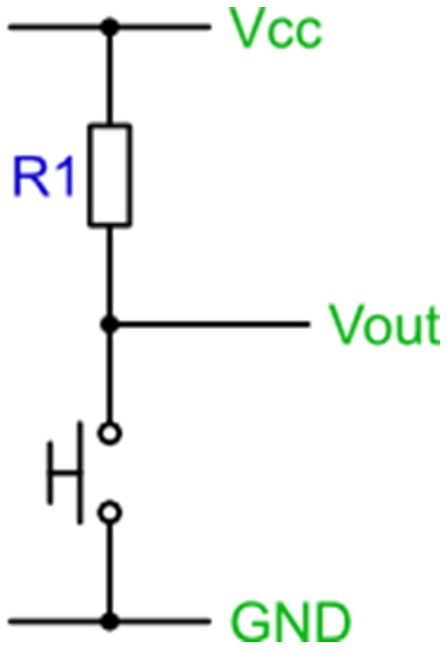
\includegraphics[width=1.00\textwidth]{switchpullupcircuit.jpg}
	\caption{Taster-Pull-Up-Schaltkreis}
	\label{fig:SwitchPullUp_Software}
\end{figure}

Der Timer-Interrupt im Mikrocontroller ruft alle 16ms eine Funktion auf, die den Taster mit einer for-Schleife entprellt. Dabei vergleicht die Funktion den alten Tastenzustand (old_button) mit dem neuen Tastenzustand (current_button) und startet nach einer Verzögerung von 10ms die Schleife erneut. Sollte der neue Tastenzustand nach 16ms immer noch der gleiche sein, wird durch eine UND-Verknüpfung vom alten Tastenzustand, dem inversen neuen Tastenzustand und der Bitmaske des Eingangs der Taster als gedrückt erkannt. Eine Erweiterung der Funktion ermöglicht das erkennen eines länger gedrückten Taster um den Zähler um zehn Einheiten zu erhöhen.
\newline